\chapter{Algorytmy śledzenia wizyjnego w robotyce mobilnej}
\label{cha:Algorymty_sledzenia_wizyjnego_w_robotyce_mobilnej}

W niniejszym rozdziale omówione szczegółowo zostaną algorytmy spotykane w literaturze w kontekście systemów śledzenia obiektów dla robotów mobilnych. Opisy konkretnych przykładów istniejących rozwiązań umieszczono w rozdziale \ref{cha:Przeglad_istniejacych_rozwiazan}. Taki podział jest dogodny, ponieważ  istniejące systemy często agregują różne algorytmy, lub wykorzystują ich zmodyfikowane wersje.

\section{Algorytm Lucasa-Kanade}
\label{sec:Algorytm_Lucasa_Kanade}
Jak wspomniano wspomniano w podrozdziale \ref{subsec:Przeplyw_optyczny} analizę ruchu zarejestrowanego w sekwencji obrazów można przeprowadzić posługując się przepływem optycznym. Takie podejście znajduje zastosowanie powszechne zastosowanie w systemach śledzenia wizyjnego, również w robotyce mobilnej. Szczególnie popularną metodą jego wyznaczania jest \textbf{algorytm Lucasa-Kanade}, wykorzystany w różnych jego odmianach w \cite{Campoy2009}, \cite{Fernandez-Caballero2010}, \cite{Liem2008}, \cite{Markovic2014}, \cite{Olivares-Mendez2009} i \cite{Sadeghi-Tehran2014}.

Zastosowanie algorytmu Lucasa-Kanade wykracza znacznie poza zagadnienie śledzenia obiektów i obejmuje między innymi mozaikowanie obrazów, obrazowanie medyczne czy rozpoznawanie twarzy \cite{Baker2004}. Sam algorytm został po raz pierwszy opublikowany w roku 1981 i od tego czasu w literaturze zaproponowano szereg jego modyfikacji.

\subsection{Klasyczny algorytm Lucasa-Kanade}
\label{subsec:Klasyczny_algorytm_Lucasa_Kanade}

Pierwsza postać algorytmu pomimo swojego wieku wciąż znajduje praktyczne zastosowanie - wykorzystano ją w rozwiązaniach \cite{Fernandez-Caballero2010} i \cite{Olivares-Mendez2009}. Oryginalną funkcją tej wersji, nazywanej czasem w literaturze addytywną \cite{Baker2004}, było dopasowanie obrazu wzorcowego $T(\vec{x})$ do obrazu wejściowego $I(\vec{x})$, gdzie $\vec{x} = (x, y)^T$ jest wektorem współrzędnych pikseli. W przypadku wyznaczania przepływu optycznego, obraz wzorcowy $T(\vec{x})$ jest podregionem obrazu z sekwencji w chwili $t = 1$, natomiast $I(\vec{x})$ jest obrazem w chwili $t = 2$ \cite{Baker2004}. Zakłada się, że wzorzec $T(\vec{x})$ uległ na obrazie $I(\vec{x})$ pewnemu sparametryzowanemu odkształceniu (ang. \textit{warp}) $\matr{W}(\vec{x}, \vec{p})$, gdzie $\vec{p}$ jest wektorem parametrów. Odkształcenie $\matr{W}(\vec{x}, \vec{p})$ przyporządkowuje pikselom wzorca $T(\vec{x})$ ich subpikselowe położenie $W(\vec{x}, \vec{p})$ w układzie współrzędnych obrazu $I$  \cite{Baker2004}, przykład przedstawiono na rysunku \ref{fig:Algorytm_Lucasa_Kanade}. Odkształcenie pomiędzy dwoma kolejnymi obrazami w sekwencji, dla których wyznaczany jest przepływ optyczny ma postać \cite{Baker2004}:
\begin{equation}
\label{equ:Odksztalcenie_przeplyw_optyczny}
	\matr{W}(\vec{x}, \vec{p}) = \begin{bmatrix}
		x + p_1 \\
		y + p_2 \\
	\end{bmatrix}
\end{equation}

\noindent
gdzie:

\begin{conditions}
	\vec{p} = (p_1, p_2)^T & przepływ optyczny \\
\end{conditions}

Zasadniczym celem algorytmu jest minimalizacja sumy kwadratów błędów pomiędzy  wzorcem $T(\vec{x})$ a odkształconym obrazem wejściowym $I(W(\vec{x}, \vec{p}))$ \cite{Baker2004}:
\begin{equation}
\label{equ:Algorytm_Lucasa_Kanade_cel}
	\sum\limits_{\vec{x}} (I(\matr{W}(\vec{x}, \vec{p})) - T(\vec{x}))^2
\end{equation}

Ponieważ przekształcenie $\matr{W}(\vec{x}, \vec{p})$ zwraca wartości subpikselowe, do wyznaczenia wartości pikseli $I(\matr{W}(\vec{x}, \vec{p}))$ konieczne jest wykonanie ich interpolacji. Wyznaczenie przepływu optycznego sprowadza się do minimalizacji wyrażenia \ref{equ:Algorytm_Lucasa_Kanade_cel} , gdzie zmienną decyzyjną jest wektor $\vec{p}$. Takie zadanie optymalizacji ma charakter nieliniowy, ponieważ pomiędzy wartościami pikseli $I(\vec{x}$ a ich współrzędnymi $\vec{x}$ nie występuje zależność liniowa (ogólnie nie występuje żadna zależność) \cite{Baker2004}. Minimalizacja jest wykonywana iteracyjnie, poprzez założenie znajomości pewnej estymacji $p$ oraz wielokrotną zmianę jej wartości o $\Delta \vec{p}$ i wyznaczenie wartości błędu dla bieżącej postaci:
\begin{equation}
\label{equ:Algorytm_Lucasa_Kanade_iteracyjnie}
	\sum\limits_{\vec{x}} (I(\matr{W}(\vec{x}, \vec{p} + \Delta \vec{p})) - T(\vec{x}))^2
\end{equation}

\begin{equation}
\label{equ:Algorytm_Lucasa_Kanade_podstawienie}
	\vec{p} \gets \vec{p} + \Delta \vec{p}
\end{equation}

Wartość $\Delta \vec{p}$ jest wyznaczana przy każdej iteracji, warunkiem zatrzymania algorytmu jest zwykle spadek pewnej jej normy $\norm{\Delta \vec{p}}$ poniżej wartości progowej $\epsilon$ \cite{Baker2004}. 

Składnik $I(\matr{W}(\vec{x}, \vec{p} + \Delta \vec{p}))$ jest linearyzowany poprzez rozwinięcie w szereg Taylora, w wyniku czego wyrażenie \ref{equ:Algorytm_Lucasa_Kanade_iteracyjnie} przyjmuje postać \cite{Baker2004}:
\begin{equation}
\label{equ:Algorytm_Lucasa_Kanade_Taylor}
	\sum\limits_{\vec{x}} (I(\matr{W}(\vec{x}, \vec{p})) + \nabla I \frac{\partial \matr{W}}{\partial \vec{p}} \Delta \vec{p} - T(\vec{x}))^2
\end{equation}

\noindent
gdzie:

\begin{conditions}
	\nabla I & gradient obrazu $\nabla I = (\frac{\partial I}{\partial x}, \frac{\partial I}{\partial y})$ \\
	\frac{\partial \matr{W}}{\partial \matr{p}} & macierz Jacobiego dla odkształcenia $\matr{W}(\vec{x}, \vec{p})$ \\
\end{conditions}

Gradient obrazu $\nabla I$ obliczany jest dla jego układu współrzędnych i odkształcany zgodnie z bieżącą estymacją $\matr{W}(\vec{x}, \vec{p})$.

\begin{figure}[!htb]
	\begin{center}
		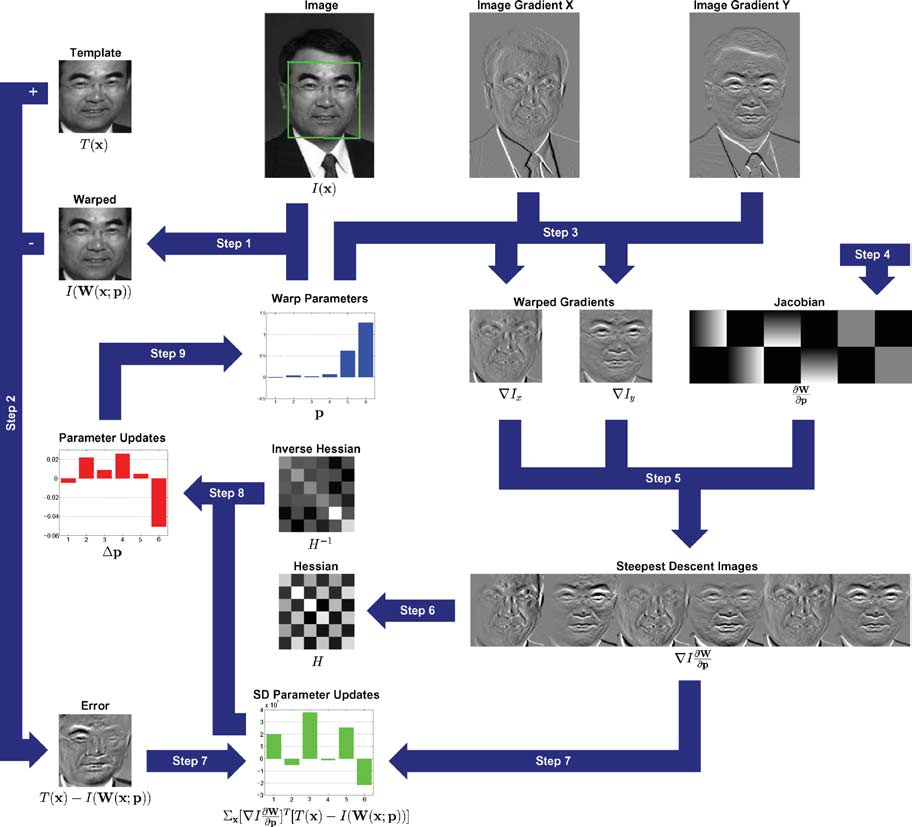
\includegraphics[width=16cm]{images/lucas_kanade_algorithm.png}
	\end{center}	
	\longcaptionsource{Przebieg algorytmu Lucasa-Kanade}{Krok 1 - wykonanie odkształcenia $W(\vec{x}, \vec{p})$ na obrazie wejściowym $I(\vec{x})$ według jego ostatniej estymacji; krok 2 - obliczenie bieżącej wartości błędu; krok 3 - wyznaczenie gradientu oraz jego odkształcenie; krok 4 - wyznaczenie macierzy Jacobiego; krok 5 - wyznaczenie $\nabla I \frac{\partial \matr{W}}{\partial \vec{p}}$; krok 6 - wyznaczenie hesjanu; krok 7 - obliczenie wartości wyrażenia $\sum\limits_{\vec{x}}(\nabla I \frac{\partial \matr{W}}{\partial \vec{p}})^T (T(\vec{x}) - I(\matr{W}(\vec{x}, \vec{p})))$; krok 8 - obliczenie zmiany wartości parametrów odkształcenia $\Delta \vec{p}$; krok 9 - uaktualnienie wektora $\vec{p}$}{\cite{Baker2004}}
\label{fig:Algorytm_Lucasa_Kanade}
\end{figure}

Znalezienie $\vec{p}$, dla którego wyrażenie \ref{equ:Algorytm_Lucasa_Kanade_Taylor} przyjmuje minimalną wartość sprowadza się do rozwiązania problemu najmniejszych kwadratów metodą Gaussa-Newtona \cite{Baker2004}. W tym celu wyznacza się jego pochodną cząstkową ze względu na $\Delta \vec{p}$ oraz porównuje się ją do zera. Po przekształceniach:
\begin{equation}
\label{equ:Algorytm_Lucasa_Kanade_Gauss_Newton}
	\Delta \vec{p} = H^{-1} \sum\limits_{\vec{x}}(\nabla I \frac{\partial \matr{W}}{\partial \vec{p}})^T (T(\vec{x}) - I(\matr{W}(\vec{x}, \vec{p})))
\end{equation}

\begin{equation}
\label{equ:Algorytm_Lucasa_Kanade_hesjan}
	H = \sum\limits_{\vec{x}}(\nabla I \frac{\partial \matr{W}}{\partial \vec{p}})^T (\nabla I \frac{\partial \matr{W}}{\partial \vec{p}})
\end{equation}

\noindent
gdzie:
\begin{conditions}
	H & aproksymacja hesjanu według metody Gaussa-Newtona \\
\end{conditions}

Cały algorytm sprowadza się do iteracyjnego wyznaczania równań \ref{equ:Algorytm_Lucasa_Kanade_Gauss_Newton} i \ref{equ:Algorytm_Lucasa_Kanade_podstawienie}. Realizację jego poszczególnych etapów przedstawiono na rysunku \ref{fig:Algorytm_Lucasa_Kanade}. Wykonanie pojedynczej iteracji ma złożoność obliczeniową $O(n^2 N + n^3)$, gdzie $N$ to liczba pikseli wzorca $T$, a $n$ to liczba parametrów odkształcenia \cite{Baker2004}.

\subsection{Algorytm Kanade-Lucasa-Tomasi}
\label{subsec:Algorytm_Kanade_Lucasa_Tomasi}

Sam algorytm Lucasa-Kanade może być w zasadzie jedynie metodą wyznaczania gęstego przepływu optycznego \cite{Yilmaz2006}. Z drugiej strony wiadomo, że pewne punkty obrazu lepiej nadają się do realizacji zadania śledzenia obiektu niż inne \cite{Tomasi1991} - dla punktów leżących na krawędziach ujawnia się problem apertury (rozdział \ref{subsec:Ruch_w_sekwencji_obrazow}), natomiast punkty leżące wewnątrz obszarów o stałej intensywności nie dostarczają żadnej informacji o ruchu. W publikacji \cite{Tomasi1991} zaproponowano metodę wyznaczenia optymalnych punktów charakterystycznych oraz ich śledzenia z wykorzystaniem algorytmu Lucasa-Kanade, nazywaną \textbf{algorytmem Kanade-Lucasa-Tomasi} (ang. \textit{Kanade-Lucas-Tomasi tracker}, w skrócie \textit{KLT}). Algorytm Lucasa-Kanade w tej postaci został zastosowany w \cite{Liem2008} i \cite{Sadeghi-Tehran2014}.

Podstawę zasady działania \textit{KLT} stanowi równanie:

\begin{equation}
\label{equ:Algorytm_Lucasa_Kanade_Tomasi_podstawowe_rówanie}
	I(x, y, t + \tau) = I(x - \xi, y - \eta, t)
\end{equation}
\noindent
gdzie:
\begin{conditions}
	I(x,y,t) & wartość piksela na obrazie $I$ o współrzędnych $(x,y)$ w chwili $t$ \\
	\tau & interwał czasowy pomiędzy dwoma klatkami \\
	\vec{d} = (\xi, \eta) & przemieszczenie punktu $\vec{x} = (x, y)$ pomiędzy klatkami $t$ i $t + \tau$ \\
\end{conditions}

Jego interpretacja jest następująca - późniejsza klatka $I(x, y, t + \tau)$ może zostać odtworzona z wcześniejszej klatki $I(x, y, t)$ poprzez odpowiednie przesunięcie jej każdego piksela, którego dla danego punktu $\vec{x}$ wynosi $\vec{d}$ (ogólnie jest to funkcja współrzędnych $(x, y)$, czasu $t$ i interwału $\tau$) \cite{Tomasi1991}. W rzeczywistości równanie \ref{equ:Algorytm_Lucasa_Kanade_Tomasi_podstawowe_rówanie} jest rzadko prawdziwe, nawet przy statycznej scenie o stałym oświetleniu \cite{Tomasi1991}.

\textit{KLT} w odróżnieniu od podstawowego algorytmu Lucasa-Kanade nie śledzi pojedynczych punktów, ale wybrane okna obrazu. Pozwala to zwiększenie odporności na szum oraz zmniejszenie prawdopodobieństwa błędnego rozpoznania punktu na kolejnym obrazie \cite{Tomasi1991}. Z drugiej strony, nie wszystkie piksele należące do konkretnego okna muszą poruszać się w jednakowy sposób (np. jeśli  okno obejmuje obszar na granicy dwóch przysłaniających się obiektów), z czym wiążą się dwa problemy: po pierwsze - jak stwierdzić, czy śledzone jest to samo okno, jeżeli jego zawartość zmienia się w czasie; po drugie - jak na podstawie informacji o prędkościach poszczególnych pikseli wnioskować o przemieszczeniu całego okna \cite{Tomasi1991}. Pierwszy problem można rozwiązać sprawdzając, jak bardzo okno zmienia się pomiędzy kolejnymi klatkami, oraz, ewentualnie, odrzucając je, jeśli zmiana jest zbyt duża. Rozwiązaniem drugiego problemu jest wprowadzenie bardziej skomplikowanego modelu zmiany okna (jak np. przekształcenia afiniczne, jak w opisanej dalej modyfikacji według \cite{Shi1994}), jednak tworzy to ryzyko nadokreślenia całego zagadnienia, ze względu na częste występowanie w sekwencjach obrazów obiektów sztywnych \cite{Tomasi1991}. Z tego powodu \textit{KLT} operuje na małych oknach, dla których wyznacza się jedynie wektor przemieszczenia, zaś każda występująca pomiędzy dwoma kolejnymi instancjami okna rozbieżność nie opisana przez niego traktowana jest jako błąd \cite{Tomasi1991}. W skutek przyjęcia założenia o małych rozmiarach okien, oryginalny algorytm \textit{KLT} nie radzi sobie w przypadku dużych przemieszczeń punktów pomiędzy klatkami.  

Przyjmując oznaczenie  $J(\vec{x}) = I(x, y, t + \tau)$, model przemieszczenia punktu pomiędzy klatkami można zdefiniować następująco:

\begin{equation}
\label{equ:Algorytm_Lucasa_Kanade_Tomasi_model}
	J(\vec{x}) = I(\vec{x} - \vec{d}) + n(\vec{x})
\end{equation}

\noindent
gdzie:
\begin{conditions}
	\vec{d} & wektor przemieszczenia punktu $\vec{d} = (\xi, \eta)$ \\
	I(\vec{x}) & Wartość piksela na obrazie $I$ o współrzędnych $\vec{x}$ w chwili $t$ \\
	n(\vec{x}) & szum \\
\end{conditions}

Z równania \ref{equ:Algorytm_Lucasa_Kanade_Tomasi_model} należy wyznaczyć wektor przemieszczenia $\vec{d}$ tak, aby zminimalizować błąd dopasowania:
\begin{equation}
\label{equ:Algorytm_Lucasa_Kanade_Tomasi_blad_dopasowania}
	\epsilon = \int_W (I(\vec{x} - \vec{d}) - J(\vec{x}))^2 w \, d\vec{x}
\end{equation}

\noindent
gdzie:
\begin{conditions}
	w & współczynnik wagowy \\
\end{conditions}

Współczynnik wagowy $w$ może być stały i wynosić $1$ lub może przyjmować wartości zgodnie z rozkładem Gaussa, w celu podkreślenia wagi centralnej części okna \cite{Tomasi1991}. Jak widać postać równania \ref{equ:Algorytm_Lucasa_Kanade_Tomasi_blad_dopasowania} jest analogiczna do bazowego równania klasycznego algorytmu Lucasa-Kanade \ref{equ:Algorytm_Lucasa_Kanade_cel}. Całe zadanie śledzenia jest wykonywane poprzez jego zastosowanie dla punktów reprezentujących środki wybranych okien.

W algorytmie \textit{KLT} zdefiniowano również metodę doboru okien dobrze nadających się do zastosowania w zadaniu śledzenia. Opiera się ona na formalnym powiązaniu właściwości macierzy $H$ z równania \ref{equ:Algorytm_Lucasa_Kanade_Gauss_Newton} dla danego punktu z właściwościami jego otoczenia \cite{Tomasi1991}. Po pierwsze, z równania \ref{equ:Algorytm_Lucasa_Kanade_Gauss_Newton} wynika wprost, że aby śledzenie było możliwe macierz $H$ musi być niezdegenerowana, w związku z czym jej wartości własne $\lambda_1$ i $\lambda_2$ muszą być większe od poziomu szumu występującego na obrazie \cite{Tomasi1991}. Po drugie, całe zadanie powinno być dobrze uwarunkowane, co oznacza, że wartości własne $\lambda_1$ i $\lambda_2$ nie powinny znacznie się od siebie różnić \cite{Tomasi1991}.

Istnieją trzy możliwe przypadki wzajemnych relacji wartości własnych macierzy $H$:
\begin{enumerate}
	\item $\lambda_1 \gg \lambda_2$ lub $\lambda_1 \ll \lambda_2$ - otoczenie punktu stanowi wzór jednokierunkowy (krawędź) i nie jest odpowiednie do śledzenia, ze względu na problem apertury (rozdział \ref{sec:Analiza_ruchu}).
	\item $\lambda_1 \approx \lambda_2 \approx 0$ - otoczenie punktu jest obszarem o stałej intensywności i nie jest odpowiednie do śledzenia, ponieważ  nie przechowuje informacji o ruchu
	\item $\lambda_1 \approx \lambda_2 \gg 0$ - otoczenie punktu jest zróżnicowane teksturowo (narożniki, wzór pieprz-sól) i dobrze nadaje się do zadania śledzenia
\end{enumerate}

W praktyce, jeżeli mniejsza wartość własna spełnia założenie o przewyższaniu poziomu szumu, cała macierz $H$ jest również dobrze uwarunkowana, co wynika z faktu ograniczenia wartości pikseli do dozwolonego przedziału \cite{Tomasi1991}. Warunek służący do poszukiwania okien odpowiednich do śledzenia można zdefiniować następująco:
\begin{equation}
\label{equ:Algorytm_Lucasa_Kanade_Tomasi_poszukiwanie_punktow}
	\min (\lambda_1, \lambda_2) > \lambda
\end{equation}

\noindent
gdzie:
\begin{conditions}
	\lambda & wartość progowa \\
\end{conditions}

Wartość progową $\lambda$ można wyznaczyć poprzez uśrednienie wyników pomiarów wartości własnych macierzy $H$ dla arbitralnie wybranych obszarów o stałej jasność (dolna granica) oraz obszarów zróżnicowanych teksturowo (górna granica) \cite{Tomasi1991}.

W publikacji \cite{Shi1994} przedstawiono ulepszenie \textit{KLT} polegające wprowadzeniu dodatkowego modelu zmiany śledzonego okna pomiędzy klatkami w postaci przekształcenia afinicznego (oryginalnie \textit{KLT} zakłada wyłącznie czystą translację). Formalnie definicja takiego modelu polega na zastąpieniu w podstawowym równaniu \ref{equ:Algorytm_Lucasa_Kanade_Tomasi_podstawowe_rówanie} wektora przesunięcia $\vec{d}$, stanowiącego czystą translację, wektorem przesunięcia $\vec{\delta}$ (określanym jako afiniczne pole ruchu) \cite{Shi1994}

\begin{equation}
\label{equ:Algorytmu_Lucasa_Kanade_Tomasi_Shi_model_afiniczny}
	\vec{\delta} = \matr{D}\vec{x} + \vec{d}
\end{equation}

\begin{equation}
\label{equ:Algorytmu_Lucasa_Kanade_Tomasi_Shi_macierz_deformacji}
	\matr{D} =
	\begin{bmatrix}
		d_{xx} & d_{xy} \\
		d_{yx} & d_{yy} \\	
	\end{bmatrix}
\end{equation}

\noindent
gdzie:
\begin{conditions}
	\matr{D} & macierz deformacji \\
	\vec{d} & wektor przesunięcia środka okna \\
\end{conditions}

Zależność pomiędzy kolejną klatką $J$ a poprzednią klatką $I$ ma postać:

\begin{equation}
\label{equ:Algorytmu_Lucasa_Kanade_Tomasi_Shi_zaleznosc_klatek}
	J(\matr{A}\vec{x} + \vec{d}) = I(\vec{x})
\end{equation}

Zadanie śledzenia polega na wyznaczeniu sześciu nieznanych parametrów, tj. elementów wektora $\vec{d}$ i macierzy $\matr{D}$, przy czym jakość ich oszacowania jest zależna od założonej wielkości okna, zróżnicowania teksturowego jego zawartości oraz rozbieżności pomiędzy klatkami (gwałtowności występującego pomiędzy nimi ruchu) \cite{Shi1994}. Im mniejsze okno, tym mniej miarodajna jest wyznaczona postać macierzy $\matr(D)$ (jej wyznaczenie jest trudniejsze przy mniejszych wariancjach ruchu), jednocześnie tym lepiej nadaje się ono do śledzenia (mniej podatne na gwałtowne zmiany zawartości \cite{Tomasi1991} \cite{Shi1994}. Śledzenie jest w związku z tym realizowane, identycznie jak w wyjściowej wersji \textit{KLT}, przy założeniu modelu ruchu w postaci czystej translacji, natomiast model ruchu w postaci przekształcenia afinicznego jest wykorzystywany do monitorowania jakości okna, poprzez porównanie jego postaci na pierwszej i bieżącej klatce \cite{Shi1994}.

\subsection{Piramidowa wersja algorytmu Lucasa-Kanade}
\label{subsec:Piramidowa_wersja_algorytmu_Lucasa_Kanade}

Wielkość śledzonego okna wpływa na dokładność i odporność algorytmu \textit{KLT} - jak wspomniano wcześniej, mniejsze okno jest mniej podatne na zachodzące w sekwencji obrazów zmiany jasności należących do niego pikseli, pozwala więc na osiągnięcie większej dokładności. Z drugiej strony zwiększenie rozmiaru okna pozwala na śledzenie bardziej gwałtownego ruchu (większych przesunięć). Rozwiązanie tego dylematu zaproponowano w \cite{Bouguet2000} - polega ona na reprezentacji obrazu w przestrzeni skali (podobnie jak w algorytmie \textit{SIFT}, \ref{subsec:Punkty_charakterystyczne}), nazywanej \textbf{piramidą obrazów} (ang. \textit{image pyramid}). Takie podejście wykorzystano w rozwiązaniu \cite{Markovic2014}.

\begin{figure}[!htb]
	\begin{center}
		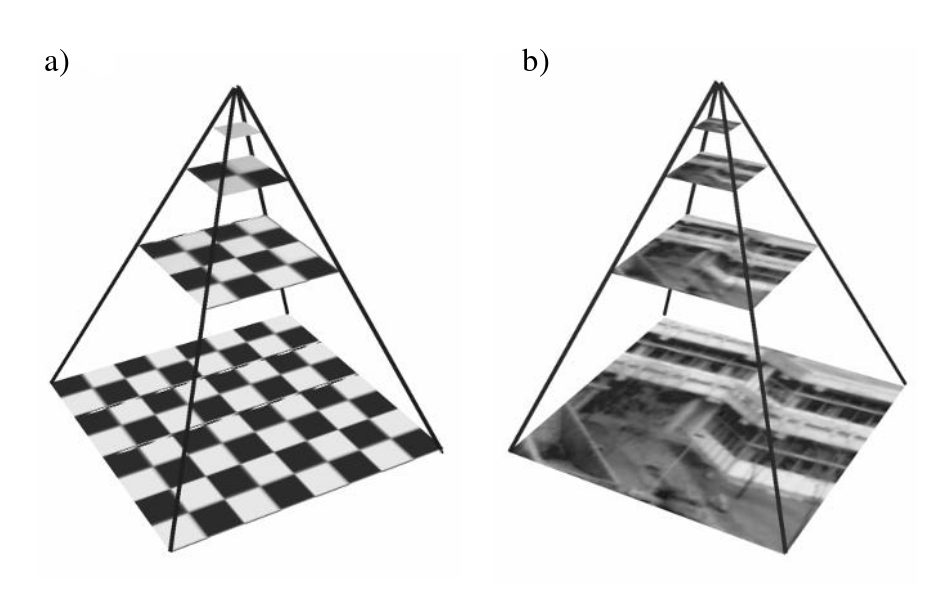
\includegraphics[width=12cm]{images/image_pyramid.png}
	\end{center}	
	\longcaptionsource{Przykłady piramidy obrazów}{Tworzenie piramidy polega na zastosowaniu rekursywnym filtrowaniu obrazu filtrem dolnoprzepustowym (wygładzającym) oraz jego podpróbkowaniu. Powyższe piramidy utworzono z wykorzystaniem filtru Gaussa. Oznaczenia: a) piramida Gaussa dla obrazu w postaci syntetycznego wzoru (szachownica), im wyższy poziom, tym bardziej ujawnia się przekłamanie początkowych wartości pikseli wnoszone przez filtrację; b) Piramida Gaussa utworzona dla rzeczywistego obrazu (zdjęcie fasady budynku)}{\cite{Jaehne2005}}
\label{fig:Przyklad_piramidy_obrazow}
\end{figure}

Obraz wejściowy $I$ ma wymiary $n_x \times n_y$, przyjęto notację, w której $I^L$ oznacza $L$-ty poziom piramidy o wymiarach $n_x^L$ i $n_y^L$, poziom zerowy to obraz nieprzeskalowany ($n_x^0 = n_x$ i $n_y^0 = n_y$). Reprezentacja piramidowa jest wyznaczana rekurencyjnie \cite{Bouguet2000}:

\begin{multline}
\label{equ:Piramidowy_algorytm_Lucasa_Kanade_piramida}
	I^L(x,y) = \frac{1}{4} I^{L-1}(2x, 2y) + \frac{1}{8}(I^{L-1}(2x - 1, 2y) + I^{L-1}(2x + 1, 2y) + I^{L-1}(2x, 2y - 1) + I^{L-1}(2x, 2y + 1)) \\ + \frac{1}{16}(I^{L-1}(2x - 1, 2y - 1) + I^{L-1}(2x + 1, 2y + 1) + I^{L-1}(2x - 1, 2y + 1) + I^{L-1}(2x + 1, 2y + 1))
\end{multline}

Równanie \ref{equ:Piramidowy_algorytm_Lucasa_Kanade_piramida} wymaga ekstrapolacji wartości skrajnych pikseli (o jednej współrzędnej równej zero) na piksle leżące poza obrazem (o jednej współrzędnej równej $-1$). Rozmiar obrazu na poziomie $L$ określany jest przez największe liczby całkowite $n_x^L$ i $n_y^L$ spełniające zależności \cite{Bouguet2000}:

\begin{equation}
\label{equ:Piramidowy_algorytm_Lucasa_Kanade_piramida_romiar_x}
	n_x^L \le \frac{n_x^{L-1} + 1}{2}
\end{equation}

\begin{equation}
\label{equ:Piramidowy_algorytm_Lucasa_Kanade_piramida_romiar_y}
	n_y^L \le \frac{n_y^{L-1} + 1}{2}
\end{equation}

Wysokość piramidy $L_m$ dobierana jest heurystycznie, przeważnie liczba poziomów nie przekracza 4 \cite{Bouguet2000}. W równaniu \ref{equ:Piramidowy_algorytm_Lucasa_Kanade_piramida} zaszyto filtr dolnoprzepustowy o masce:

\begin{equation}
\label{equ:Piramidowy_algorytm_Lucasa_Kanade_piramida_maska}
	K = \begin{bmatrix}
		1/4 & 1/2 & 1/4
	\end{bmatrix} 
	\times
	\begin{bmatrix}
		1/4 \\ 1/2 \\ 1/4
	\end{bmatrix}
\end{equation}

W praktyce stosuje się większe rozmiary maski \cite{Bouguet2000}. Wynikiem końcowym procedury jest ciąg obrazów, z których każdy jest dwukrotnie mniejszy od poprzedniego, podobny przypadek przedstawiono na rysunku \ref{fig:Przyklad_piramidy_obrazow}.

Zasadniczym celem śledzenia jest wyznaczenie dla punktu o współrzędnych $\vec{u}$ leżącego na obrazie $I$ odpowiadających mu współrzędnych $\vec{v}$ na kolejnym obrazie $J$, tzn. wyznaczenie wektora przemieszczeń $\vec{d}$, takiego że $\vec{v} = \vec{u} + \vec{d}$. Dla kolejnych poziomów piramidy obrazów $L = 0, \dots, L_m$ współrzędne punktu $\vec{u}^L = (u_x^L, u_y^L)$ wyznaczane są z zależności \cite{Bouguet2000}:

\begin{equation}
\label{equ:Piramidowy_algorytm_Lucasa_Kanade_wspolrzedne}
	\vec{u}^L = \frac{\vec{u}}{2^L}
\end{equation}

Proces śledzenia w przestrzeni skali rozpoczyna się od wyznaczenia przepływu optycznego dla najwyższego poziomu piramidy $L_m$. Jest on następnie propagowany jako początkowe przybliżenie do niższego poziomu $L_m - 1$. Na podstawie początkowego przybliżenia jest wyznaczany właściwy przepływ optyczny dla poziomu $L_m - 1$, wynik jest propagowany do poziomu $L_m -2$, itd. Rekursja kończy się po osiągnięciu poziomu 0 \cite{Bouguet2000}.

Zakładając znajomość początkowego przybliżenia przepływu optycznego $\vec{g}^L = (g_x^L, g_y^L)$ dla poziomu $L$, na podstawie obliczeń od poziomu $L_m$ do $L + 1$, w celu wyznaczenia właściwego przepływu optycznego należy znaleźć wektor $\vec{d}^L = (d_x^L, d_y^L)$, określany jako residualny przepływ optyczny, minimalizujący funkcję błędu \cite{Bouguet2000}

\begin{equation}
\label{equ:Piramidowy_algorytm_Lucasa_Kanade_blad}
	\epsilon^L(\vec{d}^L) = \sum_{x = u_x^L-\omega_x}^{u_x^L + \omega_x} \sum_{y = u_y^L-\omega_y}^{u_y^L + \omega_y} ( I^L(x,y) - J^L(x + g_x^L + d_x^L, y + g_y^L + d_y^L) )^2
\end{equation}

Zawarte w równaniu \ref{equ:Piramidowy_algorytm_Lucasa_Kanade_blad} liczby całkowite $\omega_x$ i $\omega_y$ określają rozmiar okna równy $(2\omega_x + 1) \times 2\omega_y + 1$, w obrębie którego określa się podobieństwo dla punktów $I(\vec{u})$ i $J(\vec{v})$. Wektor $\vec{d}$ wyznacza się z zastosowaniem standardowego algorytmu Lucasa-Kanade \ref{subsec:Klasyczny_algorytm_Lucasa_Kanade} \cite{Bouguet2000}. Następnie wynik jest propagowany do kolejnego poziomu $L-1$, kolejne przybliżenie początkowe $\vec{g}^{L-1}$ wyznacza się ze wzoru \cite{Bouguet2000}:

\begin{equation}
\label{equ:Piramidowy_algorytm_Lucasa_Kanade_propagacja_przeplywu}
	\vec{g}^{L-1} = 2(\vec{g}^L + \vec{d}^L)
\end{equation} 

Dla poziomu $L-1$ wyznaczany jest optymalny wektor $\vec{d}^{L-1}$ minimalizujący funkcjonał $\epsilon^{L-1}(\vec{d}^{L-1})$, następuje jego propagacja do kolejnego poziomu $L-2$ itd., aż do osiągnięcia poziomu $L = 0$. W pierwszym kroku algorytmu, w którym przetwarzany jest poziom $L_m$ jako przybliżenie początkowe $\vec{g}^{L_m}$ przyjmuje się wektor zerowy \cite{Bouguet2000}. Po wykonaniu obliczeń dla wszystkich poziomów piramidy otrzymuje się rozwiązanie końcowe:

\begin{equation}
\label{Piramidowy_algorytm_Lucasa_Kanade_wynik_koncowy}
	\vec{d} = \vec{g}^0 + \vec{d}^0 = \sum_{L = 0}^{L_m} 2^L \vec{d}^L
\end{equation}

Sens piramidowej wersji algorytmu Lucasa-Kanade leży w dekompozycji właściwego przepływu optycznego dla danego poziomu piramidy na jego znane przybliżenie $\vec{g}^L$ oraz część residualną $\vec{d}^L$ o niewielkich wartościach, które nie wzrastają przy propagacji na kolejne poziomy. Pozwala to z powodzeniem wyznaczać ich postać z wykorzystaniem klasycznego algorytmu Lucasa-Kanade, co ostatecznie skutkuje możliwością śledzenia dużych przemieszczeń $\vec{d}$. Zakładając, że algorytm Lucasa-Kanade operujący na poszczególnych poziomach piramidy może poprawnie śledzić na każdym z nich  przemieszczenie nie większe od $d_max$, ogólne maksymalne przemieszczenie dla którego wersja piramidowa działa poprawnie wynosi $d_{max final} = (2^{L_m+1}-1)$, co przy np. liczbie poziomów piramidy $L_m = 3$ daje piętnastokrotny wzrost \cite{Bouguet2000}.

\section{Filtr Kalmana}
\label{sec:Filtr_Kalmana}

\textbf{Filtr Kalmana} (ang. \textit{Kalman Filter}, w skórcie \textit{KF}) jest rekurencyjnym algorytmem optymalnej estymacji wektora stanu modelu obiektu, zakładającym jego liniowość oraz rozkład normalny amplitudy występującego szumu procesu i pomiarowego (jest rodzajem optymalnego, rekursywnego filtru Bayesa) \cite{Challa2011}. Od kiedy został po raz pierwszy opublikowany w roku 1960 znalazł szerokie zastosowanie, m.in. w systemach śledzenia obiektów \cite{Campoy2009}, \cite{Chen2009}, \cite{Kim2012}, \cite{Rui2009}, \cite{Shibata2010} i \cite{Zhao2013}. 

\subsection{Klasyczny filtr Kalmana}
\label{subsec:Klasyczny_filtr_Kalmana}

Dany jest liniowy i dyskretny układ dynamiczny opisany równaniami \cite{Welch1995}:

\begin{equation}
\label{equ:Filtr_Kalmana_rownanie_procesu}
	\vec{x}_k = \matr{A} \vec{x}_{k-1} + \matr{B} \vec{u}_{k - 1} + \vec{w}_{k-1}
\end{equation}

\begin{equation}
\label{equ:Filtr_Kalmana_rownanie_pomiaru}
	\vec{z}_k = \matr{H} \vec{x}_k + \vec{v}_k
\end{equation}

\noindent
gdzie:

\begin{conditions}
	 k & czas \\
	 \vec{x} & wektor stanu \\
	 \matr{A} & macierz przejścia, wiążąca bieżący stan z poprzednim \\
	 \matr{B} & macierz sterowania, wiążąca bieżący stan z sygnałem sterującym \\
	 \vec{u} & wektor sygnału sterującego \\
	 \vec{w} & wektor szumu procesu \\
	 \vec{z} & wektor pomiaru stanu \\
	 \matr{H} & macierz pomiaru, wiążąca wynik pomiaru ze stanem \\
	 \vec{v} & wektor szumu pomiaru \\
\end{conditions}

Szumy $\vec{w}$ i $\vec{v}$ są od siebie niezależne, mają postać postać szumu białego, a rozkład prawdopodobieństwa ich amplitud ma postać rozkładu normalnego o zerowej wartości oczekiwanej \cite{Welch1995}:

\begin{equation}
\label{equ:Filtr_Kalmana_szum_procesu}
	p(\vec{w}) = N(0, \matr{Q})
\end{equation}

\begin{equation}
\label{equ:Filtr_Kalmana_szum_pomiaru}
	p(\vec{v}) = N(0, \matr{R})
\end{equation}

\noindent
gdzie:

\begin{conditions}
	\matr{Q} & macierz kowariancji szumu procesu \\
	\matr{R} & macierz kowariancji szumu pomiarowego \\
\end{conditions}

Podsumowując, zakłada się pewną zależność pomiędzy bieżącym a poprzednim stanem obiektu, przy czym może być ona zaburzana w nieznany sposób. Stan obiektu nie jest znany, może być jedynie obserwowany za pośrednictwem pomiarów obarczonych pewnym błędem. Celem \textit{KF} jest wyznaczenie estymaty stanu tego obiektu, w sposób statystycznie optymalny ze względu na błąd estymacji.

W algorytmie \textit{KF} rozróżniono estymaty stanu \textit{a priori} $\hat{\vec{x}}_k^-$, wyznaczaną na podstawie poprzedniego stanu, oraz \textit{a posteriori} $\hat{\vec{x}}_k$, uwzględniającą ostatni wynik pomiarów. Błędy estymacji \textit{a priori} i \textit{a posteriori} definiuje się jako \cite{Welch1995}:

\begin{equation}
\label{equ:Filtr_Kalmana_blad_a_priori}
	\vec{e}_k^- \equiv \vec{x}_k - \hat{\vec{x}}_k^-
\end{equation}

\begin{equation}
\label{equ:Filtr_Kalmana_a_posteriori}
	\vec{e}_k \equiv \vec{x}_k - \hat{\vec{x}}_k
\end{equation}

Analogicznie, macierze kowariancji błędów estymacji \textit{a priori} i \textit{a posteriori} mają postaci:

\begin{equation}
\label{equ:Filtr_Kalmana_macierz_kowariancji_a_priori}
	\matr{P}_k^- = E[\vec{e}_k^- {\vec{e}_k^-}^T]
\end{equation}

\begin{equation}
\label{equ:Filtr_Kalmana_macierz_kowariancji_a_posteriori}
	\matr{P}_k = E[\vec{e}_k \vec{e}_k^T]
\end{equation}

\noindent
gdzie:

\begin{conditions}
	E & operator wartości oczekiwanej \\
\end{conditions}

Elementy macierzy kowariancji błędów leżące na ich głównych przekątnych to wariancje błędów estymacji poszczególnych zmiennych stanu, stanowiące miarę niepewności tej estymacji. Pozostałe elementy to kowariancje pomiędzy błędami estymacji poszczególnych zmiennych stanu, określające ich wzajemne powiązanie. Na podstawie estymaty \textit{a priori} można wyznaczyć estymatę \textit{a posteriori}, zgodnie z zależnością \cite{Welch1995}:

\begin{equation}
\label{equ:Filtr_Kalmana_wyznaczenie_estymaty_a_posteriori}
	\hat{\vec{x}}_k = \hat{\vec{x}}_k^- + \matr{K}(\vec{z}_k - \matr{H}\hat{\vec{x}}_k^-)
\end{equation}

\noindent
gdzie:

\begin{conditions}
	K & macierz wzmocnienie Kalmana \\
\end{conditions}

Macierz wzmocnienia Kalmana $\matr{K}$ powinna być zostać określona tak, aby minimalizować wariancję \textit{a posteriori} $\matr{P}_k$, jedna z jej możliwych postaci może zostać obliczona z równania \cite{Welch1995}:

\begin{equation}
\label{equ:Filtr_Kalmana_wzmocnienie_Kalmana}
	\matr{K}_k = \matr{P}_k^- \matr{H}^T ( \matr{H} \matr{P}_k^- \matr{H}^T +\matr{R} ) ^ {-1}
\end{equation}

Z równania \ref{equ:Filtr_Kalmana_wzmocnienie_Kalmana} wynika, że im bardziej elementy macierzy kowariancji błędu pomiarowego $\matr{H}$ zbliżają się do zera, tym bardziej wynik równania \ref{equ:Filtr_Kalmana_wyznaczenie_estymaty_a_posteriori} zależy od wyniku pomiaru $\vec{z}_k$ i jednocześnie mniej zależy od estymaty \textit{a priori} $\hat{\vec{x}}_k^-$. Z drugiej strony, dążenie wartości elementów macierzy kowariancji błędów estymacji \textit{a priori} do zera implikuje spadek znaczenia pomiaru $\vec{z}_k$ i wzrost znaczenia przewidywanego wyniku $\hat{\vec{x}}_k^-$ \cite{Welch1995}.

Algorytm estymacji stanu z wykorzystaniem \textit{KF} składa się dwóch etapów. Pierwszy z nich, określany jako faza predykcji, polega na wyznaczeniu nowej estymaty stanu oraz macierzy kowariancji błędów \textit{a priori} na podstawie ich poprzednich postaci \cite{Welch1995}:

\begin{equation}
\label{equ:Filtr_Kalmana_faza_predykcji_stan}
	\hat{\vec{x}}_k^- = \matr{A} \hat{\vec{x}}_{k-1} + \matr{B} \vec{u}_{k - 1}
\end{equation}

\begin{equation}
\label{equ:Filtr_Kalmana_faza_predykcji_macierz_kowariancji_bledow}
	\matr{P}_k^- = \matr{A} \matr{P}_{k-1} \matr{A}^T + \matr{Q}
\end{equation}

W pierwszy kroku zakłada się początkowe wartości $\hat{\vec{x}}_{k-1}$ oraz $\matr{P}_{k-1}$. Po fazie predykcji następuje faza korekcji, w której uwzględniając wyniki pomiarów wyznacza się wartości \textit{a posteriori} \cite{Welch1995}:

\begin{equation}
\label{equ:Filtr_Kalmana_faza_korekcji_wzmocnienie}
	\matr{K}_k = \matr{P}_k^- \matr{H}^T ( \matr{H} \matr{P}_k^- \matr{H}^T +\matr{R} ) ^ {-1}
\end{equation}

\begin{equation}
\label{equ:Filtr_Kalmana_faza_korekcji_stan}
	\hat{\vec{x}}_k = \hat{\vec{x}}_k^- + \matr{K}_k(\vec{z}_k - \matr{H}\hat{\vec{x}}_k^-)
\end{equation}

\begin{equation}
\label{equ:Filtr_Kalmana_faza_korekcji_macierz_kowariancji_bledow}
	\matr{P}_k = (\matr{I} - \matr{K}_k \matr{H}) \matr{P}_k^-
\end{equation}

Po zakończeniu iteracji wartości \textit{a posteriori} traktowane są jako wartości \textit{a priori} dla kolejnego kroku $k+1$. Macierz kowariancji szumu pomiarowego $\matr{R}$ można zwykle wyznaczyć eksperymentalnie. Bardziej kłopotliwe jest określenie postaci macierzy kowariancji szumu procesu $\matr{Q}$. Przy założeniu dużej dokładności pomiarów przyjęcie dużych wartości elementów $\matr{Q}$, a więc dużej niepewności procesu, może przynieść zadowalające rezultaty. Innym rozwiązaniem jest wykonanie identyfikacji systemu poprzez dobór wartości macierzy $\matr{R}$ i $\matr{Q}$ z wykorzystaniem np. drugiego filtru Kalmana \cite{Welch1995}.

\subsection{Rozszerzony filtr Kalmana}
\label{subsec:Rozszerzony_filtr_Kalmana}

Jak wspomniano wcześniej, zastosowanie \textit{KF} w klasycznej postaci ogranicza się do układów liniowych. W przypadku układów nieliniowych (opisanych równaniami \ref{equ:Rozszerzony_Filtr_Kalmana_rownanie_procesu} i \ref{equ:Rozszerzony_Filtr_Kalmana_rownanie_pomiaru}) znajduje zastosowanie jego zmodyfikowana wersja, nosząca nazwę \textbf{rozszerzonego filtru Kalmana} (ang. \textit{Extended Kalman Filter}, w skrócie \textit{EKF}) \cite{Welch1995}.

\begin{equation}
\label{equ:Rozszerzony_Filtr_Kalmana_rownanie_procesu}
	\vec{x}_k = f(\vec{x}_{k-1}, \vec{u}_{k-1}, \vec{w_{k-1}})
\end{equation}

\begin{equation}
\label{equ:Rozszerzony_Filtr_Kalmana_rownanie_pomiaru}
	\vec{z}_k = h(\vec{x}_k, \vec{v}_k)
\end{equation}

\noindent
gdzie:

\begin{conditions}
	 f & nieliniowa funkcja wiążąca bieżący stan ze stanem poprzednim, sygnałem sterowania oraz szumem procesu \\
	 h & nieliniowa funkcja wiążąca wynik pomiaru ze stanem oraz szumem pomiarowym \\
\end{conditions}

Ponieważ konkretne wartości szumów $\vec{w_k}$ i $\vec{v_k}$ nie są znane, wektor stanu oraz wektor wyników pomiarów można aproksymować przez ich pominięcie \cite{Welch1995}:

\begin{equation}
\label{equ:Rozszerzony_Filtr_Kalmana_rownanie_procesu_aproksymacja}
	\tilde{\vec{x}}_k = f(\hat{\vec{x}}_{k-1}, \vec{u_{k-1}}, 0)
\end{equation}

\begin{equation}
\label{equ:Rozszerzony_Filtr_Kalmana_rownanie_pomiaru_aproksymacja}
	\tilde{\vec{z}}_k = h(\tilde{x}_k, 0)
\end{equation}

\noindent
gdzie:

\begin{conditions}
	 \tilde{\vec{x}}_k & aproksymacja wektora stanu w chwili $k$ \\
	 \tilde{\vec{z}}_k & aproksymacja wyników pomiarów w chwili $k$ \\
	 \hat{\vec{x}}_k & estymata stanu \textit{a posteriori} z poprzedniego kroku $k$
\end{conditions}

Istotną wadą \textit{EKF} jest brak zachowania normalnego rozkładu szumów po poddaniu ich nieliniowym przekształceniom \cite{Welch1995}. W celu dokonania estymacji wykonywana jest linearyzacja równań \ref{equ:Rozszerzony_Filtr_Kalmana_rownanie_pomiaru} i \ref{equ:Rozszerzony_Filtr_Kalmana_rownanie_procesu} poprzez ich rozwinięcie w szereg Taylora w otoczeniu przybliżeń \ref{equ:Rozszerzony_Filtr_Kalmana_rownanie_procesu_aproksymacja} i \ref{equ:Rozszerzony_Filtr_Kalmana_rownanie_pomiaru_aproksymacja} \cite{Welch1995}:

\begin{equation}
\label{equ:Rozszerzony_Filtr_Kalmana_rownanie_procesu_Taylor}
	\vec{x}_k \approx \tilde{\vec{x}}_k + \matr{A}_k(\vec{x}_{k-1} - \hat{\vec{x}}_{k-1}) + \matr{W}_k\vec{w}_{k-1}
\end{equation}

\begin{equation}
\label{equ:Rozszerzony_Filtr_Kalmana_rownanie_pomiaru_Taylor}
	\vec{z}_k \approx \tilde{\vec{z}}_k + \matr{H}_k(\vec{x}_k - \tilde{x}_k) + \matr{V}_k\vec{v}_k
\end{equation}

\noindent
gdzie:

\begin{conditions}
	\matr{A}_k & macierz Jacobiego pochodnych cząstkowych funkcji $f$ ze względu na $\vec{x}$ w chwili $k$ \\
	\matr{W}_k & macierz Jacobiego pochodnych cząstkowych funkcji $f$ ze względu na $\vec{w}$ w chwili $k$ \\
	\matr{H}_k & macierz Jacobiego pochodnych cząstkowych funkcji $h$ ze względu na $\vec{x}$ w chwili $k$ \\
	\matr{V}_k & macierz Jacobiego pochodnych cząstkowych funkcji $h$ ze względu na $\vec{v}$ w chwili $k$ \\
\end{conditions}

\noindent
Elementy macierzy $\matr{A}_k$, $\matr{W}_k$, $\matr{H}_k$ i $\matr{V}_k$ zdefiniowane są następująco:

\begin{equation}
\label{equ:Rozszerzony_Filtr_Kalmana_macierz_A}
	\matr{A}_{k,[i,j]} = \frac{\partial f_{[i]}}{\partial \vec{x}_{[j]}} (\hat{\vec{x}}_{k-1}, \vec{u}_{k-1}, 0)
\end{equation}

\begin{equation}
\label{equ:Rozszerzony_Filtr_Kalmana_macierz_W}
	\matr{W}_{k,[i,j]} = \frac{\partial f_{[i]}}{\partial \vec{w}_{[j]}} (\hat{\vec{x}}_{k-1}, \vec{u}_{k-1}, 0)
\end{equation}

\begin{equation}
\label{equ:Rozszerzony_Filtr_Kalmana_macierz_H}
	\matr{H}_{k,[i,j]} = \frac{\partial h_{[i]}}{\partial \vec{x}_{[j]}} (\tilde{\vec{x}}_k, 0)
\end{equation}

\begin{equation}
\label{equ:Rozszerzony_Filtr_Kalmana_macierz_V}
	\matr{V}_{k,[i,j]} = \frac{\partial h_{[i]}}{\partial \vec{v}_{[j]}} (\tilde{\vec{x}}_k, 0)
\end{equation}

\noindent
Zakłada się definicję błędów przybliżeń wektora stanu $\tilde{\vec{e}}_{\vec{x}_k}$ i pomiarów $\tilde{\vec{e}}_{\vec{z}_k}$:

\begin{equation}
\label{equ:Rozszerzony_Filtr_Kalmana_blad_stanu}
	\tilde{\vec{e}}_{\vec{x}_k} \equiv \vec{x}_k - \tilde{\vec{x}}_k
\end{equation}

\begin{equation}
\label{equ:Rozszerzony_Filtr_Kalmana_blad_pomiaru}
	\tilde{\vec{e}}_{\vec{z}_k} \equiv \vec{z}_k - \tilde{\vec{z}}_k
\end{equation}

Po wstawieniu równań \ref{equ:Rozszerzony_Filtr_Kalmana_blad_stanu} i \ref{equ:Rozszerzony_Filtr_Kalmana_blad_pomiaru} do równań \ref{equ:Rozszerzony_Filtr_Kalmana_rownanie_procesu_Taylor} i \ref{equ:Rozszerzony_Filtr_Kalmana_rownanie_pomiaru_Taylor} przekształceniach \cite{Welch1995}:

\begin{equation}
\label{equ:Rozszerzony_Filtr_Kalmana_blad_stanu_cd}
	\tilde{\vec{e}}_{\vec{x}_k} \approx \matr{A}_k(\vec{x}_{k-1} - \hat{\vec{x}}_{k-1}) + \vec{\epsilon}_k
\end{equation}

\begin{equation}
\label{equ:Rozszerzony_Filtr_Kalmana_blad_pomiaru_cd}
	\tilde{\vec{e}}_{\vec{z}_k} \approx \matr{H}_k \tilde{\vec{e}}_{\vec{x}_k} + \vec{\eta}_k
\end{equation}

\noindent
gdzie:

\begin{conditions}
	\vec{\epsilon}_k & niezależna zmienna losowa o zerowej wartości średniej i macierzy kowariancji $\matr{W}\matr{Q}_k\matr{W}^T$ \\
	\vec{\eta}_k & niezależna zmienna losowa o zerowej wartości średniej i macierzy kowariancji $\matr{V}\matr{R}_k\matr{V}^T$ \\
\end{conditions}

Równania \ref{equ:Rozszerzony_Filtr_Kalmana_blad_stanu_cd} i \ref{equ:Rozszerzony_Filtr_Kalmana_blad_pomiaru_cd} są liniowe i mają podobną postać jak równania procesu \ref{equ:Filtr_Kalmana_rownanie_procesu} i pomiaru \ref{equ:Filtr_Kalmana_rownanie_pomiaru} \textit{KF}, co sugeruje wykorzystanie drugiego, hipotetycznego filtru Kalmana do estymacji błędu predykcji $\tilde{\vec{e}}_{\vec{x}_k}$ \cite{Welch1995}. Jego estymacja, oznaczona jako $\hat{\vec{e}}_k$, może następnie służyć do wyznaczenia estymaty stanu \textit{a posteriori} układu nieliniowego, na podstawie równania \ref{equ:Rozszerzony_Filtr_Kalmana_blad_stanu}:

\begin{equation}
\label{equ:Rozszerzony_Filtr_Kalmana_estymacja_stanu}
	\hat{\vec{x}}_k = \tilde{\vec{x}}_k + \hat{\vec{e}}_k
\end{equation}

Zmienne losowe $\vec{\epsilon}_k$ i $\vec{\eta}_k$ mają w przybliżeniu rozkłady prawdopodobieństwa odpowiednio $p(\vec{\epsilon}_k) \sim N(0, \matr{W}\matr{Q}_k\matr{W}^T)$ i $p(\vec{\eta}_k) \sim N(0, \matr{V}\matr{R}_k\matr{V}^T)$. Korzystając z równania \ref{equ:Filtr_Kalmana_wyznaczenie_estymaty_a_posteriori}, oraz zakładając zerową wartość predykcji $\hat{\vec{e}}_k$ \cite{Welch1995}:

\begin{equation}
\label{equ:Rozszerzony_Filtr_Kalmana_estymacja_bledu}
	\hat{\vec{e}}_k = \matr{K}_k \tilde{\vec{e}}_{\vec{z}_k}
\end{equation}

Wstawienie równania \ref{equ:Rozszerzony_Filtr_Kalmana_estymacja_bledu} do \ref{equ:Rozszerzony_Filtr_Kalmana_estymacja_stanu} oraz podstawienie aproksymowanej wartości błędu pomiaru na postawie równania \ref{equ:Rozszerzony_Filtr_Kalmana_blad_pomiaru} ujawnia brak konieczności stosowania drugiego \textit{KF} i pozwala na wyznaczenie postaci równania korekcji stanu \textit{EKF} \cite{Welch1995}:

\begin{equation}
\label{equ:Rozszerzony_Filtr_Kalmana_estymacja_stanu_cd}
	\hat{\vec{x}}_k = \tilde{\vec{x}}_k + \matr{K}_k (\vec{z}_k - \tilde{\vec{z}}_k)
\end{equation}

Macierz wzmocnienia Kalmana $\matr{K}_k$ wyznacza się analogicznie jak w \textit{KF}, na podstawie równania \ref{equ:Filtr_Kalmana_faza_korekcji_macierz_kowariancji_bledow}, podstawiając zmodyfikowaną postać macierzy kowariancji błędów pomiaru.

Równania \textit{EKF} fazy predykcji przyjmują następującą postać \cite{Welch1995}:

\begin{equation}
\label{equ:Rozszerzony_Filtr_Kalmana_faza_predykcji_stan}
	\hat{\vec{x}}_k^- = f(\vec{x}_{k-1}, \vec{u}_{k-1}, 0)
\end{equation}

\begin{equation}
\label{equ:Rozszerzony_Filtr_Kalmana_faza_predykcji_macierz_kowariancji_bledow}
	\matr{P}_k^- = \matr{A}_k \matr{P}_{k-1} \matr{A}_k^T + \matr{W}_k\matr{Q}_{k-1}\matr{W}_k^T
\end{equation}

Równania fazy korekcji \cite{Welch1995}:

\begin{equation}
\label{equ:Rozszerzony_Filtr_Kalmana_faza_korekcji_wzmocnienie}
	\matr{K}_k = \matr{P}_k^- \matr{H}_k^T ( \matr{H}_k \matr{P}_k^- \matr{H}_k^T + \matr{V}_k\matr{R}_k\matr{V}_k^T ) ^ {-1}
\end{equation}

\begin{equation}
\label{equ:Rozszerzony_Filtr_Kalmana_faza_korekcji_stan}
	\hat{\vec{x}}_k = \hat{\vec{x}}_k^- + \matr{K}_k(\vec{z}_k - h(\hat{\vec{x}}_k^-,0))
\end{equation}

\begin{equation}
\label{equ:Rozszerzony_Filtr_Kalmana_faza_korekcji_macierz_kowariancji_bledow}
	\matr{P}_k = (\matr{I} - \matr{K}_k \matr{H}_k) \matr{P}_k^-
\end{equation}

\section{Algorytm Mean Shift}
\label{Algorytm_Mean_Shift}

